Im praktischen Durchlauf verbleiben auch im letzten Bild aus Abbildung \ref{img:imageTree} noch schwache horizontale Streifen.
Das liegt an den Ungenauigkeiten im Prüfprozess und der Mustererzeugung (vgl. Abschnitt \ref{sub:unterschiedeKameraUndMonitor}).
Da das Ergebnis mit weiteren phasenverschobenen Streifenmustern stetig besser wird, könnte man diese durch eine höhere Anzahl von Streifenmustern $N_{shift}$ eliminieren.
Dabei gilt zu beachten, dass man im Diskreten und Numerischen arbeitet und bei einer sehr hohen Anzahl von Phasenverschiebungen Messfehler und Gleitpunktfehler zum Tragen kommen.
Das bedeutet, man muss eine zum Prüfaufbau passende Anzahl an Mustern verwenden, um bessere Ergebnisse dokumentieren zu können.
Zur Bildverbesserung hat man auch die Möglichkeit, die zuvor erwähnte Fourier-Analyse anzuwenden.
Die noch verbliebenen Strukturen lassen sich im Amplitudenspektrum des Bildes durch die Ausbreitungsrichtung finden.
Da diese Strukturen nur noch sehr schwach im Bild vorhanden ist, sind die jeweiligen Frequenzkomponenten auch dementsprechend gering gewichtet (siehe Abbildung \ref{img:amplitudeSpectrum}).

\begin{figure}[H]
	\centering
	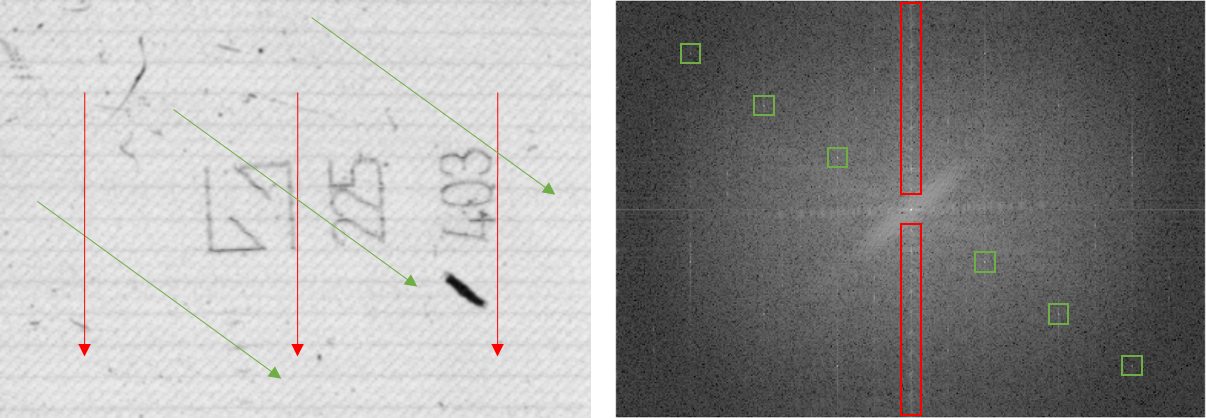
\includegraphics[width=\textwidth]{03_sichtpruefungDurchLichtstreuung/optimierungen/figures/amplitudeSpectrum}
	\caption[Amplitudenspektrum des Gesamtbildes]{Amplitudenspektrum des Gesamtbildes. (mit Markierungen)}
	\label{img:amplitudeSpectrum}
\end{figure}

\noindent
In Rot ist im Bild die Ausbreitungsrichtung der ersten Struktur markiert, die entsprechenden Gewichte der Frequenzkomponenten sind in derselben Farbe im Amplitudenspektrum gezeichnet.
Analog sind in Grün die für die zweite Struktur relevante Ausbreitungsrichtung und Gewichte der Frequenzkomponenten markiert.
Die grün gekennzeichnete Struktur entsteht in diesem Fall durch die Verwendung eines speziellen Polfilters auf dem Objektiv der Kamera, auf dessen Funktion nicht genauer eingegangen werden muss.
Filtert man im Amplitudenspektrum die markierten Bereiche heraus und wendet die inverse Fourier-Transformation an, erhält man ein Bild, indem die beiden störenden Strukturen nicht mehr vorhanden sind.
Das Ergebnisbild wird durch ein geeignetes Werkzeug \cite{fourierTool} berechnet und in Abbildung \ref{img:frequencyFiltered} dargestellt.

\begin{figure}[H]
	\centering
	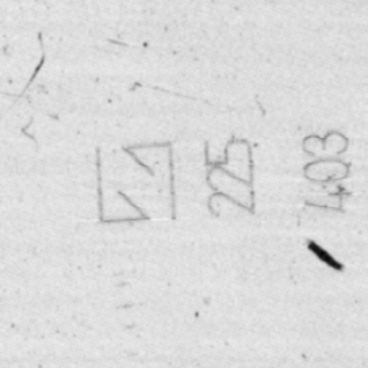
\includegraphics[width=0.4\textwidth]{03_sichtpruefungDurchLichtstreuung/optimierungen/figures/frequencyFiltered}
	\caption[Bild mit angewandtem frequenzselektives Filter]{Angewandtes frequenzselektives Filter nach Abbildung \ref{img:amplitudeSpectrum}. Erstellt mit dem Online-Werkzeug \glqq Fourifier\grqq ~von © 2020 Ejectamenta.\cite{fourierTool}\footnotemark}
	\label{img:frequencyFiltered}
\end{figure}
\footnotetext{Anmerkungen: Das Bild musste aufgrund der Anforderungen des verwendeten Online-Werkzeugs zugeschnitten werden. Außerdem wurden die Frequenzkomponenten \glqq händisch\grqq ~entfernt, weshalb das Bild fehlerbehaftet ist. Das Bild konnte auch nicht auf Korrektheit geprüft werden und dient nur der Veranschaulichung. Die Nutzungsrechte unterliegen der Lizenz von © 2020 Ejectamenta. Für weitere Informationen zu Geschäfts- und Nutzungsbedingungen siehe: \url{https://ejectamenta.com/about/terms-of-service/}}